\section{Rotating frames of reference}
Recall that Newton's laws are only valid in \textit{inertial} frames. A rotating frame is non-inertial and therefore the equation of motion needs to be modified.

Let $S$ is an inertial frame and $S'$ a rotating frame about the $z$-axis in $S$ with angular velocity $ \omega $. Denote the basis vectors for $S$ as 
\[
    \bfe_i = \{\hat{\bfx},\hat{\bfy},\hat{\bfz}\},
\]
and for $S'$ 
\[
    \bfe_i' = \{\hat{\bfx}',\hat{\bfy}',\hat{\bfz}'\}.
\]
Consider a particle at rest in $S'$. Its velocity viewed in $S$ is 
\[
    \left( \frac{\mathrm{d}\bfr}{\mathrm{d}t}  \right)_S = \boldsymbol{\omega} \times \mathbf{r},\quad \text{where $ \boldsymbol{\omega}=\omega \hat{\bfz} $}.
\]
The angular velocity vector is aligned with the axis of rotation, and with the magnitude equal to scalar angular velocity. In convention, $z$-axis is chosen so that viewed from the direction of the angular velocity, the rotation is anti-clockwise.

Same formula applies to any vector fixed in $S'$, in particular to the basis vectors $ \bfe_i' $:
\[
    \left( \frac{\mathrm{d}\bfe_i'}{\mathrm{d}t}  \right)_S = \boldsymbol{\omega}\times \bfe_i'.
\]

Consider a general time-dependent vector $ \mathbf{a} $. In $ S' $ we can write
\[
    \mathbf{a}(t) = \sum_{i=1}^{3} a_i'(t)\bfe_i'(t).
\]
Now consider rate of change of $ \mathbf{a} $:
\[
    \left( \frac{\mathrm{d}\bfa(t)}{\mathrm{d}t}  \right)_{S'} = \sum_{i=1}^{3}\frac{\mathrm{d}(a_i'(t))}{\mathrm{d}t}\bfe_i'(t) ,
\] 
and in $S$ 
\begin{align*}
    \left( \frac{\mathrm{d}\bfa(t)}{\mathrm{d}t} \right)_S 
    &= \sum_{i=1}^{3}\frac{\mathrm{d}(a_i'(t))}{\mathrm{d}t}\bfe_i'(t) + \sum_{i=1}^{3} a_i'(t) \left( \frac{\mathrm{d}}{\mathrm{d}t}\bfe_i'(t) \right)_S \\ 
    &= \left( \frac{\mathrm{d}\bfa(t)}{\mathrm{d}t}  \right)_{S'}+\boldsymbol{\omega} \times \bfa.
\end{align*}
Applying to position vector $\bfr$  gives
\[
    \left( \frac{\mathrm{d}\bfr(t)}{\mathrm{d}t} \right)_S=\left( \frac{\mathrm{d}\bfr(t)}{\mathrm{d}t}  \right)_{S'}+\boldsymbol{\omega}\times \bfr.
\]
Note that the difference depends on position. Now apply the same identity to velocity(assume $ \boldsymbol{\omega} $ is time-dependent):
\begin{align*}
    \left( \frac{\mathrm{d}^2\bfr}{\mathrm{d}t^2}  \right)_S &= \left( \left( \frac{\mathrm{d}}{\mathrm{d}t}  \right)_{S'}+\boldsymbol{\omega}\times  \right)\left( \left( \frac{\mathrm{d}}{\mathrm{d}t}  \right)_{S'}+\boldsymbol{\omega}\times  \right)\bfr\\ 
    &=\left( \frac{\mathrm{d}^2\bfr}{\mathrm{d}t^2}  \right)_{S'}+2 \boldsymbol{\omega}\times \left( \frac{\mathrm{d}\bfr}{\mathrm{d}t}  \right)_{S'}+\dot{\boldsymbol{\omega}}\times \mathbf{r}+\boldsymbol{\omega} \times (\boldsymbol{\omega} \times \mathbf{r}).
\end{align*}
Therefore the equation of motion in a rotating frame is 
\begin{align*}
    &m \left( \frac{\mathrm{d}^2\bfr}{\mathrm{d}t^2}  \right)_S =\bfF\\ 
    \Longrightarrow &\bfF= m\left( \left( \frac{\mathrm{d}^2\bfr}{\mathrm{d}t^2}  \right)_{S'}+2 \boldsymbol{\omega}\times \left( \frac{\mathrm{d}\bfr}{\mathrm{d}t}  \right)_{S'}+\dot{\boldsymbol{\omega}}\times \mathbf{r}+\boldsymbol{\omega} \times (\boldsymbol{\omega} \times \mathbf{r}) \right).
\end{align*}
Need to take account of fictitious forces to explain motion observed in the rotating frame:
\begin{enumerate}[align=left]
    \item[\textbf{Coriolis force}:] $\displaystyle -2m\boldsymbol{\omega}\times \left( \frac{\mathrm{d}\bfr}{\mathrm{d}t}  \right)_{S'}$.
    \item[\textbf{Euler force}:] $\displaystyle -m\dot{\boldsymbol{\omega}}\times \mathbf{r}$, in many applications, take this to be zero.
    \item[\textbf{Centrifugal force}:] $\displaystyle -m\boldsymbol{\omega} \times (\boldsymbol{\omega} \times \mathbf{r})$.
\end{enumerate}

\subsection{Centrifugal force}
The centrifugal force is given by 
\begin{align*}
    -m\boldsymbol{\omega} \times (\boldsymbol{\omega} \times \mathbf{r}) &= -m((\boldsymbol{\omega}\cdot \mathbf{r})\boldsymbol{\omega}-\boldsymbol{\omega}^2 \mathbf{r})\\ 
    &= m \omega^2(\bfr - \hat{\boldsymbol{\omega}}(\hat{\boldsymbol{\omega}} \cdot \mathbf{r}))\\ 
    &= m \omega^2 \mathbf{r}_{\perp}
\end{align*}
where $ \hat{\boldsymbol{\omega}} $ is a unit vector in the direction of $ \boldsymbol{\omega} $ and $ \mathbf{r}_{\perp } $ is the perpendicular component of $ \mathbf{r} $ relative to $ \boldsymbol{\omega} $. Note that $ |\mathbf{r}_{\perp }|  $ is the perpendicular distance from the point mass to the axis of rotation.
\begin{center}
    \begin{tikzpicture}
        \draw [->] (0,-1) -- (0,2) node [pos=1,above] {$ \boldsymbol{\omega} $};
        \node [left] (0) at (0,-0.5) {$O$};
        \node [dot] (1) at (0,-0.5) {};
        \node [dot] (2) at (1.5,1) {};
        \draw [dashed, ->-=0.6] (1) -- (2) node [below right, pos=0.5] {$ \mathbf{r} $};
        \draw [dashed,->-=0.6] (0,1) -- (2) node [pos=0.5,above] {$ \mathbf{r}_{\perp } $};
        \draw [dashed] (0,1) ellipse (1.5 and 0.35);
    \end{tikzpicture}
\end{center}
Note that
\begin{align*}
    & \mathbf{r}_\perp^2 = r^2-(\boldsymbol{\omega}\cdot \mathbf{r})^2 = |\boldsymbol{\omega}\times \mathbf{r}|^2\\ 
    \Longrightarrow & \nabla \mathbf{r}_\perp^2 = r \mathbf{r} - 2 \boldsymbol{\omega} (\boldsymbol{\omega}\cdot \mathbf{r}) = 2 \mathbf{r}_\perp.
\end{align*}
Hence 
\[
    m \omega^2 \mathbf{r}_{\perp} = \nabla \left( \frac{1}{2}m \omega^2 \mathbf{r}_\perp^2 \right),
\]
centrifugal force is \textit{conservative}. 

On a rotating planet, it is convenient to combine centrifugal force and gravitational force into ``effective gravity'' $ \mathbf{g}_{\text{eff}}=\mathbf{g}+\omega^2 \mathbf{r}_\perp  $. Consider the following diagram of a planet:
\begin{center}
    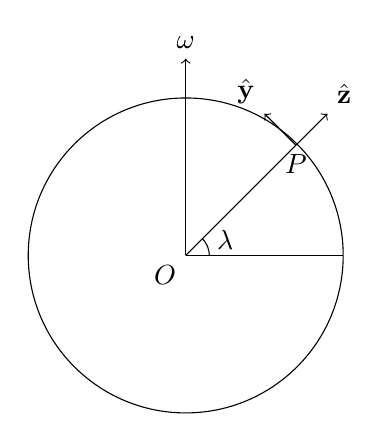
\begin{tikzpicture}
      \draw circle [radius = 2];
      \node [anchor = north east] {$O$};
      \draw [->] (0, 0) -- (0, 2.5) node [above] {$\boldsymbol\omega$};
      \draw (0, 0) -- (2, 0);
      \draw (0, 0) -- (1.4, 1.4) node [below] {$P$};
      \draw [->] (1.4, 1.4) -- (1.8, 1.8) node [anchor = south west] {$\hat{\mathbf{z}}$};
      \draw [->] (1.4, 1.4) -- (1, 1.8) node [anchor = south east] {$\hat{\mathbf{y}}$};
      \draw (0.3, 0) arc (0:45:0.3);
      \node at (0.5, 0.2) {$\lambda$};
    \end{tikzpicture}
\end{center}

Note that $ \hat{\bfx} $ is horizontal and \textit{eastward} (i.e. points inside the paper), $ \hat{\bfy} $ is horizontal and northward, and $ \hat{\bfz} $ is vertical. At $P$,
\begin{align*}
    \mathbf{r} &= R\hat{\mathbf{z}}\\
    \boldsymbol\omega &= \omega(\cos\lambda \hat{\mathbf{y}} + \sin \lambda \hat{\mathbf{z}})\\
    \mathbf{g} &= -g\hat{\mathbf{z}}\\
\end{align*}
Now 
\begin{align*}
    \mathbf{g}_{\text{eff}} &= -g \hat{\bfz}+ \omega^2 \mathbf{r}_\perp\\ 
    &=  -g \hat{\bfz}+ \omega^2 R \cos \lambda(\hat{\bfz} \cos \lambda-\hat{\bfy}\sin \lambda)\\
    &= \hat{\bfz}(\omega^2 R \cos^2 \lambda-g)- \hat{\bfy}\omega^2 R \cos \lambda \sin \lambda.
\end{align*}
The angle between $ \mathbf{g}_{\text{eff}} $ and $ \hat{\bfz} $ is 
\[
    \alpha = \arctan \left( \frac{\omega^2 R \cos \lambda \sin \lambda}{g-\omega^2 R \cos^2 \lambda} \right).
\]
For Earth, $ \omega=\frac{2\pi}{86400\rms}\approx 7.3 \times 10^{-5}\rms^{-1},R \approx 6.4 \times 10^6 \rmm $, so $ \omega^2 R/g \approx 3.5 \times 10^{-3} $ and $ \alpha $ is very small.
\subsection{Coriolis force}\
Recall that Coriolis force is given by 
\[
    -2m\boldsymbol{\omega}\times \left( \frac{\mathrm{d}\bfr}{\mathrm{d}t}  \right)_{S'} = -2m \boldsymbol{\omega} \times \mathbf{v},
\]
where $ \mathbf{v} $ is the velocity observed in $ S' $. Observe that this force is \textit{proportional} to the velocity, \textit{perpendicular} to the velocity (in $S'$), and it does not do work.

Consider Coriolis force on a rotating planet, and consider the velocity \textit{tangential} to surface: $ \mathbf{v} = v_x \hat{\bfx}+ v_y \hat{\bfy} $. Note that $ \boldsymbol{\omega}=\omega( \cos \lambda \hat{\bfy}+ \sin \lambda \hat{\bfz}) $. Hence 
\[
    -2m \boldsymbol{\omega}\times \mathbf{v} = 2m\omega \sin \lambda \left( v_y \hat{\bfx}-v_x \hat{\bfy} \right)+2m\omega \cos \lambda v_x \hat{\bfz}.
\]
The horizontal Coriolis force gives an acceleration to the \textit{right} of velocity in \textit{nothern hemisphere}, and to the \textit{left} in \textit{southern hemisphere}. Note that it can be balanced by another force, e.g. pressure gradient.

\begin{example}
    Suppose a ball is dropped from a tower of height $h$ at the equator. Where does it land?

    In the rotating frame,
    \[
      \ddot{\mathbf{r}} = \mathbf{g} - 2\boldsymbol\omega\times \dot{\mathbf{r}} - \boldsymbol\omega\times(\boldsymbol\omega\times \mathbf{r}).
    \]
    We work to first order in $\omega$\footnote{Since the Earth is rotating slow, $ \omega^2R/g $ is small and it makes sense to neglect higher orders.}. Then
    \[
      \ddot{\mathbf{r}} = \mathbf{g} - 2\boldsymbol\omega\times \dot{\mathbf{r}} + O(\omega^2).
    \]
    Integrate wrt $t$ to obtain
    \[
      \dot{\mathbf{r}} = \mathbf{g}t - 2\boldsymbol\omega \times (\mathbf{r} - \mathbf{r}_0) + O(\omega^2),
    \]
    where $\mathbf{r}_0$ is the initial position. We substitute into the original equation to obtain
    \[
      \ddot{\mathbf{r}} = \mathbf{g} - 2\boldsymbol\omega\times \mathbf{g}t + O(\omega^2).
    \]
    (where some new $\omega^2$ terms are thrown into $O(\omega^2)$). We integrate twice to obtain
    \[
      \mathbf{r} = \mathbf{r}_0 + \frac{1}{2}\mathbf{g}t^2 - \frac{1}{3}\boldsymbol\omega \times \mathbf{g}t^3 + O(\omega^2).
    \]
    In components, we have $\mathbf{g} = (0, 0, -g)$, $\boldsymbol\omega = (0, \omega, 0)$ and $\mathbf{r}_0 = (0, 0, R + h)$. So
    \[
      \mathbf{r} = \left(\frac{1}{3}\omega gt^3, 0, R + h - \frac{1}{2}gt^2\right) + O(\omega^2).
    \]
    So the particle hits the ground at $t = \sqrt{2h/g}$ and its eastward displacement is
    \[
        \frac{1}{3}wg\left(\frac{2h}{g}\right)^{3/2}.
    \]
  
    This can be understood in terms of angular momentum conservation in the non-rotating frame. At the beginning, the particle has the same angular velocity with the Earth. As it falls towards the Earth, to maintain the same angular momentum, the angular velocity has to increase to compensate for the decreased radius. So it spins faster than the Earth and drifts towards the East, relative to the Earth.
\end{example}

\begin{example}[Foucault pendulum]
    Consider a pendulum that is free to swing in any plane, e.g.\ a weight on a string. At the North pole, it will swing in a plane that is fixed in an inertial frame, while the Earth rotates beneath it. From the perspective of the rotating frame, the plane of the pendulum rotates backwards. This can be explained as a result of the Coriolis force.
    In general, at latitude $\lambda$, the plane rotates rightwards with period $\frac{1\text{ day}}{\sin \lambda}$.
\end{example}